\documentclass[12pt,a4paper]{ctexart}

\usepackage[a4paper,margin=2.5cm]{geometry}
\usepackage{setspace}
\usepackage{array}
\usepackage{longtable}
\usepackage{graphicx}
\usepackage{fancyhdr}
\usepackage{titling}
\usepackage{enumitem}
\usepackage{amsmath,amssymb}
\usepackage{booktabs}
\usepackage{caption}
\usepackage{float}
\usepackage{bm}
\usepackage{hyperref}
\usepackage{listings}
\usepackage[dvipsnames,svgnames,x11names]{xcolor}

\lstset{
	backgroundcolor=\color[rgb]{0.96,0.96,0.96},
	keywordstyle=\color{blue}\bfseries,
	identifierstyle=\color{black},
	commentstyle=\color[rgb]{0,0.6,0},
	stringstyle=\color[rgb]{0.58,0,0.82},
	basicstyle=\small\ttfamily,
	columns=fullflexible,
	breaklines=true,
	captionpos=t,
	tabsize=4,
	emph={self},
	emphstyle=\bfseries\color{Rhodamine},
	frame=lines,
	framesep=1em,
	rulesepcolor=\color{red!20!green!20!blue!20},
	language=Python,
	numbers=left,
	showstringspaces=false,
	numberstyle=\footnotesize,
	extendedchars=false,
	xleftmargin=3em
}

\setlength{\parindent}{2em}
\setlength{\parskip}{0.5em}
\renewcommand{\arraystretch}{1.5}
\linespread{1.3}

\pagestyle{fancy}
\fancyhf{}
\cfoot{\thepage}
\renewcommand{\headrulewidth}{0pt}

% ===== 可修改信息 =====
\newcommand{\schoolname}{数学与统计学院}
\newcommand{\classname}{数学强基2301}
\newcommand{\studentid}{2233210080}
\newcommand{\studentname}{袁浩然}
\newcommand{\teachername}{孟德宇老师}
\newcommand{\labplace}{数学实验中心}
\newcommand{\experimenttitle}{实验六：基于 VAE 的艺术风格迁移与生成}
\newcommand{\schoolyear}{2023--2024学年\quad 第二学期}
\usepackage{fancyhdr}

% 设置 fancyhdr 样式
\fancypagestyle{plain}{
	\fancyhf{} % 清除所有预设的页眉和页脚
	\renewcommand{\headrulewidth}{0pt} % 如果不需要页眉线
	\renewcommand{\footrulewidth}{0pt} % 如果不需要页脚线
}

% 应用新的 plain 样式到所有页面
\pagestyle{plain}

\begin{document}

\section*{\experimenttitle}

\section*{一、实验内容}
本实验围绕变分自编码器（Variational Autoencoder, VAE）展开，目标是利用 COCO 写实照片和 WikiArt 印象派画作构建双域图像数据集，在统一分辨率与归一化预处理的基础上，训练 VAE 模型完成图像重建、双向风格迁移、潜在空间插值和随机图像生成。具体任务包括：
\begin{enumerate}[label=(\arabic*)]
    \item 准备两类图像数据，其中写实照片取自 COCO 的 \texttt{val2014} 文件夹，艺术图像取自筛选后的 \texttt{wikiart\_subset} 文件夹，并统一调整为 $256\times 256$；
    \item 按照 $8:1:1$ 的比例划分训练集、验证集和测试集，并将像素值归一化到 $[0,1]$ 区间；
    \item 基于 PyTorch 构建包含编码器、重参数化模块和解码器的 VAE 网络，采用 Adam 优化器训练 50 轮，并引入早停策略；
    \item 利用编码器得到潜在向量，在潜在空间中实现照片域与艺术域之间的迁移、插值和随机采样生成；
    \item 从定量和定性两个角度分析模型效果，其中定量指标重点考察重建误差（MSE），并预留 FID 的计算接口。
\end{enumerate}

\section*{二、实验原理}

\subsection*{1. VAE 的基本思想}
普通自编码器通过编码器将输入样本压缩到低维表示，再通过解码器恢复原始图像；而 VAE 在此基础上进一步假设潜在变量服从某种概率分布。对于输入图像 $x$，编码器不直接输出固定隐变量，而是输出潜在分布的均值和对数方差：
\[
q_{\phi}(z|x)=\mathcal{N}(z;\mu(x),\sigma^2(x)).
\]
为了保证网络可训练，VAE 采用重参数化技巧：
\[
z=\mu+\sigma\odot\varepsilon,\qquad \varepsilon\sim \mathcal{N}(0,I).
\]
这样既能保留随机性，又能通过反向传播更新网络参数。

\subsection*{2. 损失函数}
本实验采用“重建损失 + KL 散度损失”的组合形式：
\[
\mathcal{L}=\mathcal{L}_{\text{recon}}+\beta\,\mathcal{L}_{\text{KL}}.
\]
其中：
$$\mathcal{L}_{\text{recon}} = \|x-\hat{x}\|_1,\ \mathcal{L}_{\text{KL}} = -\frac{1}{2}\sum_{i=1}^{d}\left(1+\log\sigma_i^2-\mu_i^2-\sigma_i^2\right).$$
重建损失衡量生成图像与原图之间的差异，KL 散度用于约束潜在分布接近标准正态分布，从而提高生成能力与潜在空间的连续性。训练时引入 $\beta$ 的逐步升温（KL warmup）策略，有助于缓解训练初期图像过度模糊的问题。

\subsection*{3. 风格迁移与潜在空间插值}
VAE 的一个重要优点是潜在空间具有较好的连续性和可解释性。本实验中，一张写实照片经过编码器得到潜在向量后，可以通过解码器输出具有艺术域特征的结果；反过来，艺术图像也可以映射回写实风格。此外，给定两类图像的潜在向量 $z_p$ 和 $z_a$，还可以通过
\[
z_{\alpha}=(1-\alpha)z_p+\alpha z_a,\qquad \alpha\in[0,1]
\]
构造过渡风格图像。当从标准正态分布中随机采样潜在变量 $z\sim\mathcal{N}(0,I)$ 时，解码器还能生成全新的风格化图像。

\section*{三、数据准备与预处理}
本实验使用两个文件夹中的图像作为输入数据：
\begin{itemize}
    \item \texttt{val2014}：COCO 日常场景照片；
    \item \texttt{wikiart\_subset}：从 WikiArt 中筛选出的印象派画作子集。
\end{itemize}
根据实验要求，最终选取 10000 张写实照片和 8000 幅印象派画作，并确保两类图像覆盖人物、风景、建筑等多种典型场景。所有图像统一缩放为 $256\times 256$，使用 \texttt{ToTensor()} 将像素从 $0\sim255$ 映射到 $[0,1]$ 区间。

在数据集划分时，分别对两个域独立进行随机打乱，并按照 $8:1:1$ 的比例划分为训练集、验证集和测试集。代码中训练集使用随机翻转增强，以提升模型的泛化能力；验证集与测试集仅做尺度变换与归一化，不引入随机扰动。

\section*{四、模型结构与训练设置}

\subsection*{1. 网络结构}
本实验代码采用卷积 VAE 结构。编码器由多层卷积块组成，每层使用卷积、批归一化和 LeakyReLU 激活，将输入图像逐步压缩为高维特征表示；随后通过两个全连接层分别输出潜在变量的均值 $\mu$ 和对数方差 $\log\sigma^2$。解码器由全连接层和多层反卷积块组成，最终恢复出 $256\times256$ 的 RGB 图像。

为了更好地区分写实域和艺术域，代码中在解码阶段引入了域嵌入向量（domain embedding），使得解码器能够根据目标域标签输出不同风格的图像。这样不仅能够实现同域重建，还能支持照片到印象派、印象派到写实图像的双向迁移。

\subsection*{2. 超参数设置}
实验的主要训练参数如下：
\begin{center}
\begin{tabular}{cc}
\toprule
参数 & 取值 \\
\midrule
输入分辨率 & $256\times256$ \\
潜在变量维度 & 192 \\
批大小 & 16 \\
学习率 & $2\times10^{-4}$ \\
训练轮数 & 50 \\
早停轮数 & 10 \\
优化器 & Adam \\
最大 KL 权重 $\beta_{\max}$ & 0.01 \\
KL warmup 轮数 & 10 \\
\bottomrule
\end{tabular}
\end{center}

\subsection*{3. 训练流程}
训练阶段将两个域的数据拼接形成联合训练集。每个 batch 输入网络后，先由编码器得到潜在分布参数，再经重参数化得到隐变量，最后结合域标签送入解码器输出重建结果。程序在每个 epoch 后统计训练集与验证集上的总损失、重建损失和 KL 损失，并保存验证集性能最优的模型参数到 \texttt{best\_cvae.pth}。当验证损失连续多轮不再下降时，触发早停，防止模型过拟合。

\section*{五、核心代码说明}
下面给出与实验最相关的几段代码。The code of the task is available at \footnote{https://github.com/HaoranYuandomestic/ex6\_VAE.git}

\subsection*{1. 数据集读取与预处理}
\begin{lstlisting}
class ImageDomainDataset(Dataset):
    def __init__(self, paths, domain_label, train=False):
        self.paths = paths
        self.domain_label = domain_label
        if train:
            self.transform = transforms.Compose([
                transforms.Resize((cfg.image_size, cfg.image_size)),
                transforms.RandomHorizontalFlip(p=0.5),
                transforms.ToTensor(),
            ])
        else:
            self.transform = transforms.Compose([
                transforms.Resize((cfg.image_size, cfg.image_size)),
                transforms.ToTensor(),
            ])

    def __getitem__(self, idx):
        img = Image.open(self.paths[idx]).convert("RGB")
        img = self.transform(img)
        return img, self.domain_label
\end{lstlisting}
这一部分负责从文件夹中读取图片，同时为每张样本附加域标签：\texttt{0} 表示写实照片域，\texttt{1} 表示印象派艺术域。

\subsection*{2. 编码器、重参数化与解码器}
\begin{lstlisting}
class ConditionalVAE(nn.Module):
    def __init__(self, latent_dim=192, domain_emb_dim=16):
        super().__init__()
        self.encoder = nn.Sequential(
            ConvBlock(3, 32), ConvBlock(32, 64), ConvBlock(64, 128),
            ConvBlock(128, 256), ConvBlock(256, 256), ConvBlock(256, 512)
        )
        self.fc_mu = nn.Linear(512 * 4 * 4, latent_dim)
        self.fc_logvar = nn.Linear(512 * 4 * 4, latent_dim)
        self.domain_emb = nn.Embedding(2, domain_emb_dim)
        self.fc_decode = nn.Linear(latent_dim + domain_emb_dim, 512 * 4 * 4)
\end{lstlisting}
在解码时，潜在变量与域嵌入向量拼接后再送入解码器，这使得模型具备了双域生成能力。

\subsection*{3. 损失函数与训练}
\begin{lstlisting}
def vae_loss(recon, x, mu, logvar, beta):
    recon_loss = F.l1_loss(recon, x, reduction="mean")
    kl = -0.5 * torch.mean(torch.sum(1 + logvar - mu.pow(2) - logvar.exp(), dim=1))
    total = recon_loss + beta * kl
    return total, recon_loss, kl
\end{lstlisting}
训练过程中记录总损失、重建损失和 KL 损失，并通过验证集损失判断是否保存最佳模型与执行早停。

\section*{六、实验结果与可视化分析}
程序训练完成后，将主要结果统一保存到 \texttt{visualizations} 文件夹中。结合当前文件夹中的输出文件，可以从以下几个方面分析模型性能。

\subsection*{1. 输入样本示意}
图 \ref{fig:input-samples} 给出了测试阶段从两个域中取出的示例图像。可以看出，写实照片与印象派画作在纹理、色彩分布和边缘平滑程度上存在明显差异，这为跨域迁移提供了基础。

\begin{figure}[H]
    \centering
    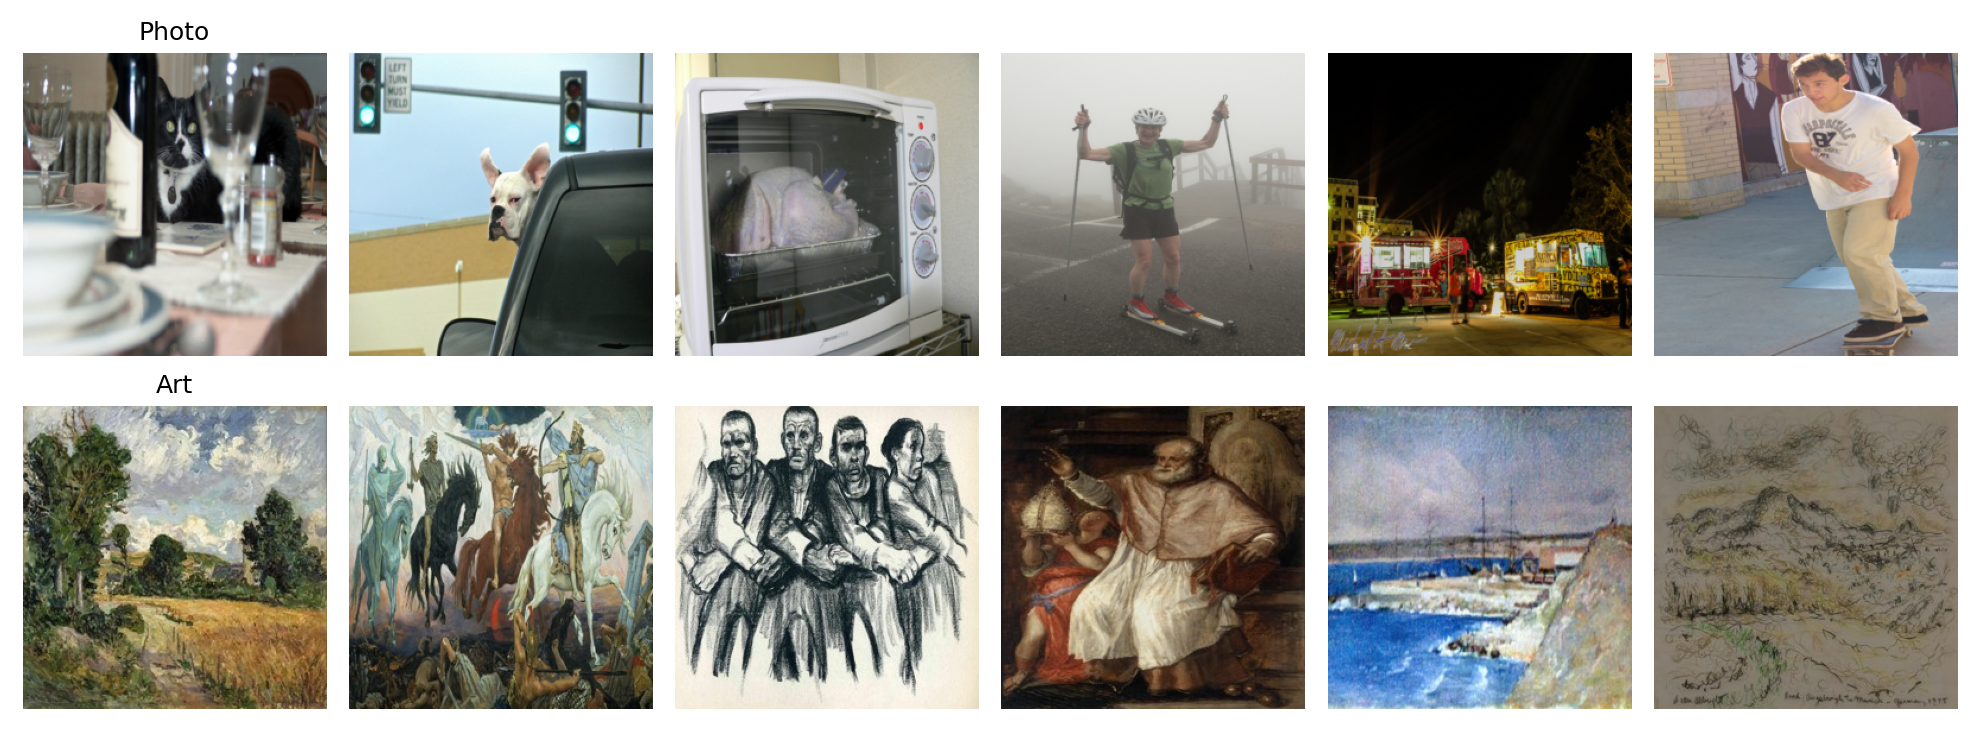
\includegraphics[width=0.95\textwidth]{visualizations/input_samples.png}
    \caption{写实照片域与印象派艺术域输入样本}
    \label{fig:input-samples}
\end{figure}

\subsection*{2. 训练损失与 KL 曲线}
图 \ref{fig:loss-curve} 展示了训练集与验证集上的总损失变化趋势。整体来看，随着 epoch 增加，模型损失逐步下降并趋于平稳，说明 VAE 已经学到有效的图像压缩与重建表示。图 \ref{fig:kl-curve} 展示了 KL 项的变化，它在 warmup 阶段逐步增长，说明潜在空间分布约束在训练后期开始发挥作用。

\begin{figure}[H]
    \centering
    
\includegraphics[width=0.8\textwidth]{visualizations/loss_curve.png}
    \caption{训练集与验证集损失曲线}
    \label{fig:loss-curve}
\end{figure}

\begin{figure}[H]
    \centering
    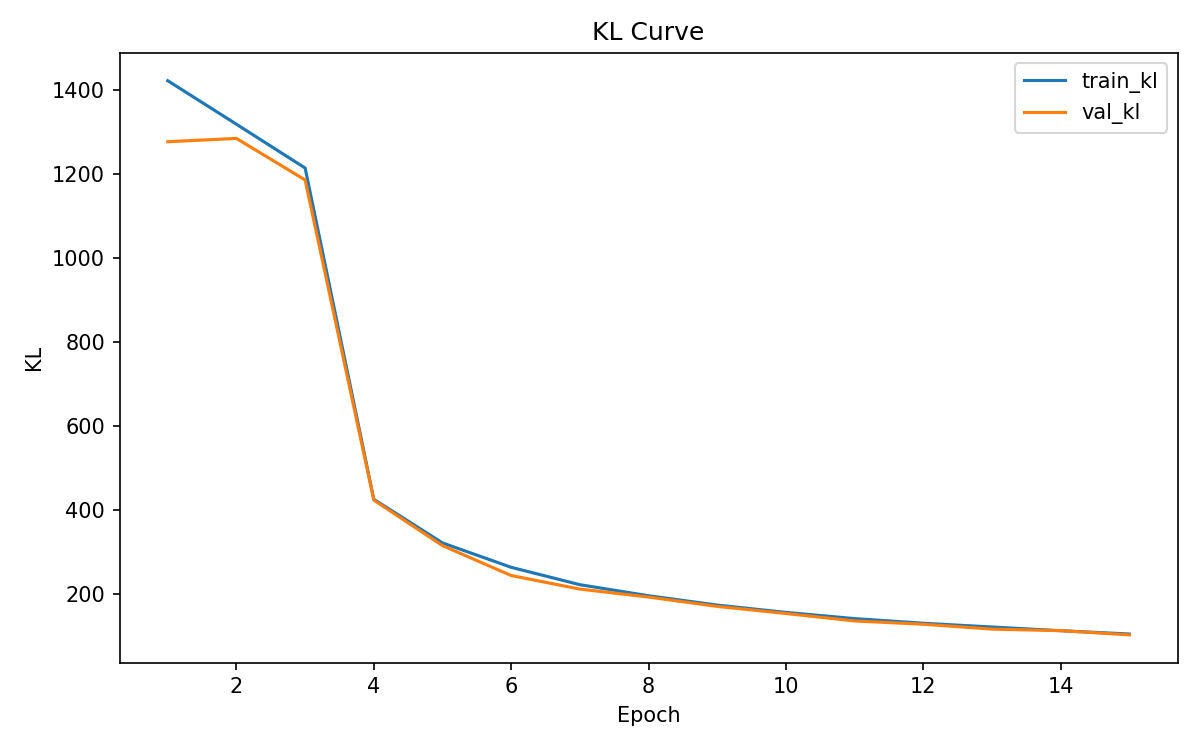
\includegraphics[width=0.8\textwidth]{visualizations/kl_curve.png}
    \caption{KL 损失曲线}
    \label{fig:kl-curve}
\end{figure}

\subsection*{3. 图像重建效果}
图 \ref{fig:recon} 展示了写实照片与艺术图像各自经过编码、采样与解码后的重建结果。可以看到，模型较好地保留了原图的整体布局、主体位置和主要颜色分布，但在细节纹理和边缘锐度上仍有一定损失，这也是 VAE 相比 GAN 类模型较常见的现象。

\begin{figure}[H]
    \centering
    
\includegraphics[width=0.95\textwidth]{visualizations/reconstruction_compare.png}
    \caption{照片域与艺术域的输入图像及重建图像对比}
    \label{fig:recon}
\end{figure}

\subsection*{4. 双向风格迁移结果}
图 \ref{fig:transfer} 是本实验最核心的结果之一。上半部分展示了写实照片输入后输出为印象派风格图像的结果，下半部分展示了艺术图像输入后恢复到写实域的结果。可以发现，模型在保持基本构图不变的前提下，对颜色饱和度、笔触平滑感和局部纹理进行了明显转换，说明条件 VAE 已经学到了一定程度的域间映射关系。

\begin{figure}[H]
    \centering
    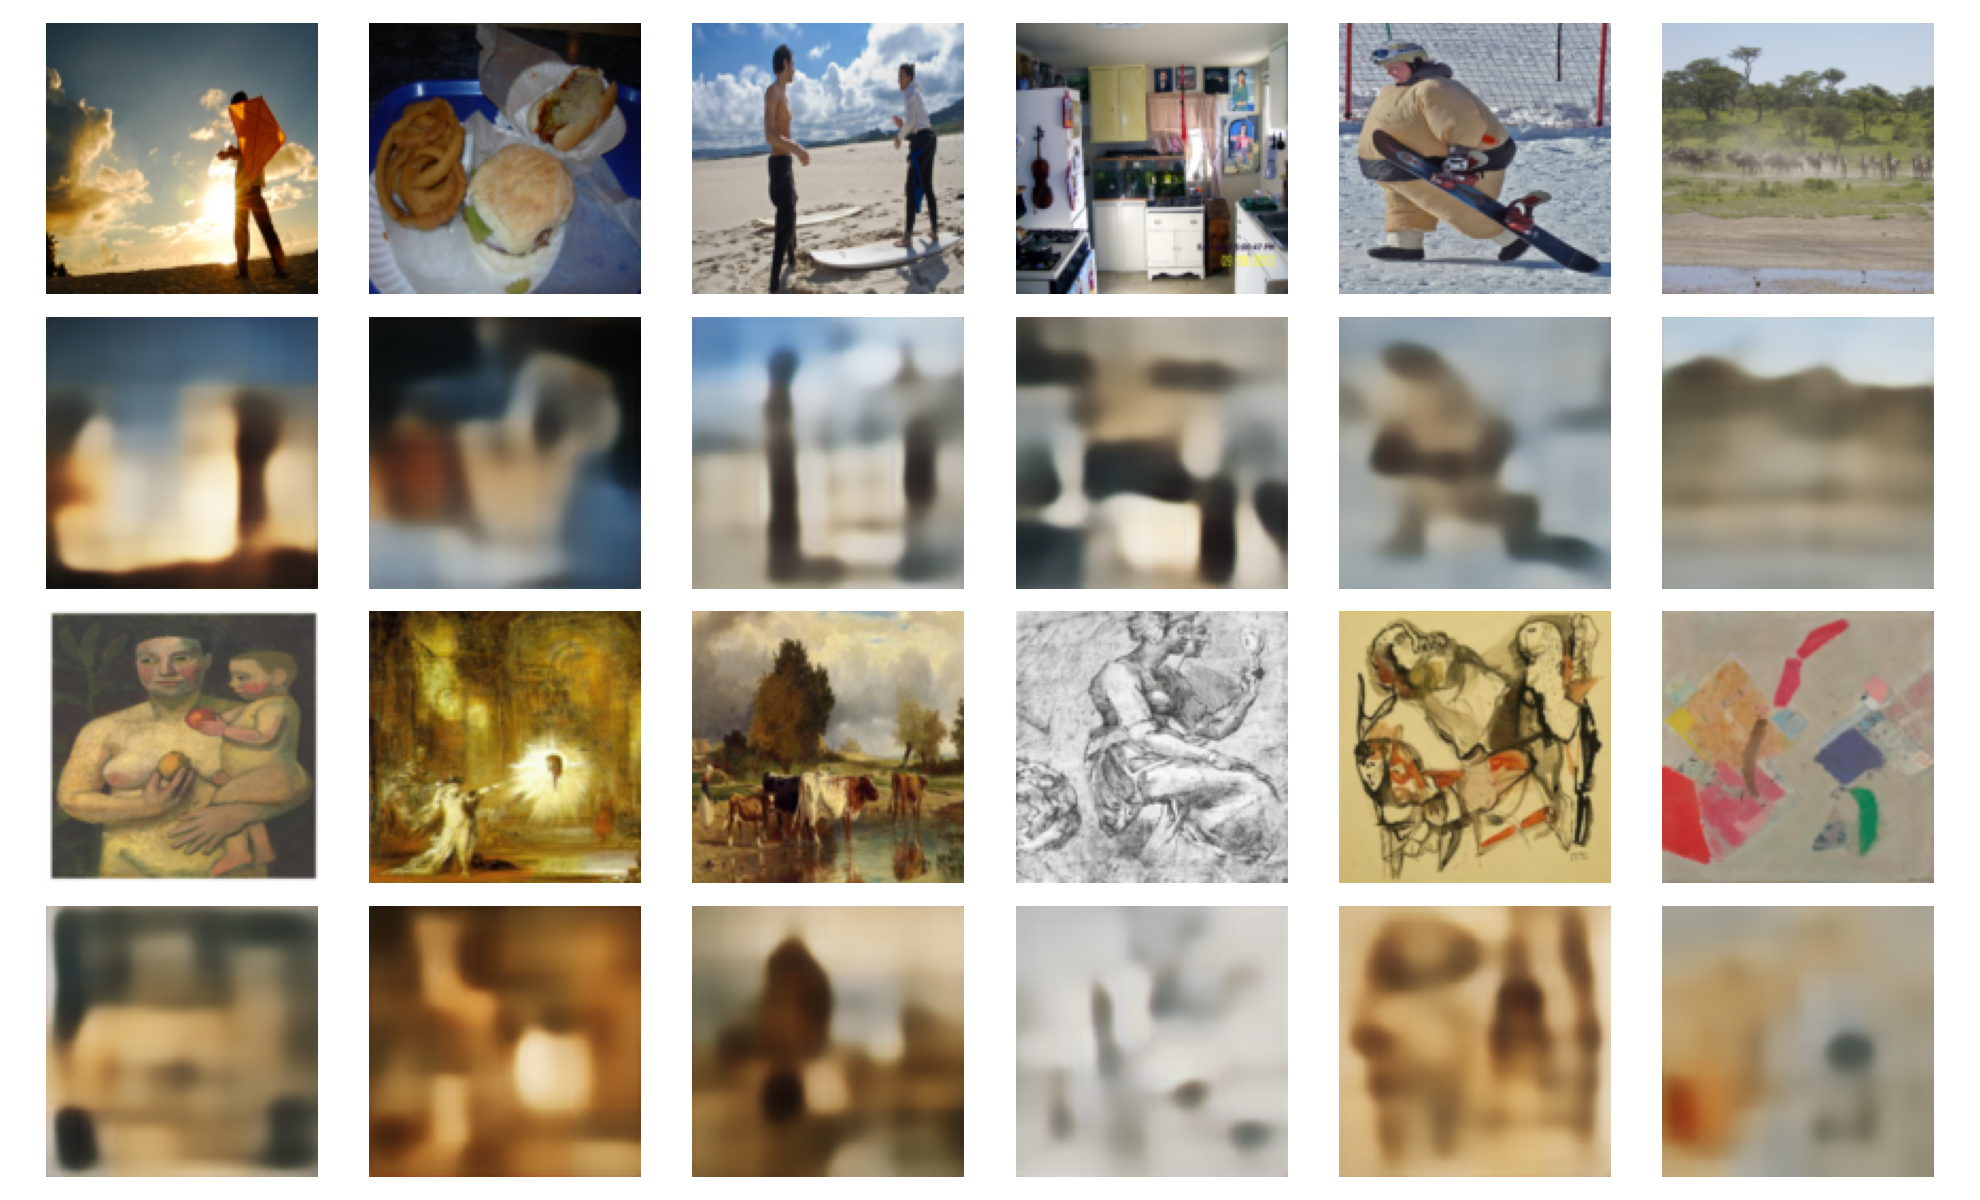
\includegraphics[width=0.95\textwidth]{visualizations/style_transfer_bidirectional.png}
    \caption{双向风格迁移结果：Photo$\rightarrow$Art 与 Art$\rightarrow$Photo}
    \label{fig:transfer}
\end{figure}

\subsection*{5. 潜在空间插值}
图 \ref{fig:interp} 展示了在一张写实照片和一张印象派画作之间进行潜在向量线性插值的结果。从左到右，随着插值系数 $\alpha$ 从 0 逐渐增大到 1，图像风格呈现出连续、平滑的变化趋势，这反映出 VAE 学到的潜在空间具有一定的流形结构与连续性。

\begin{figure}[H]
    \centering
    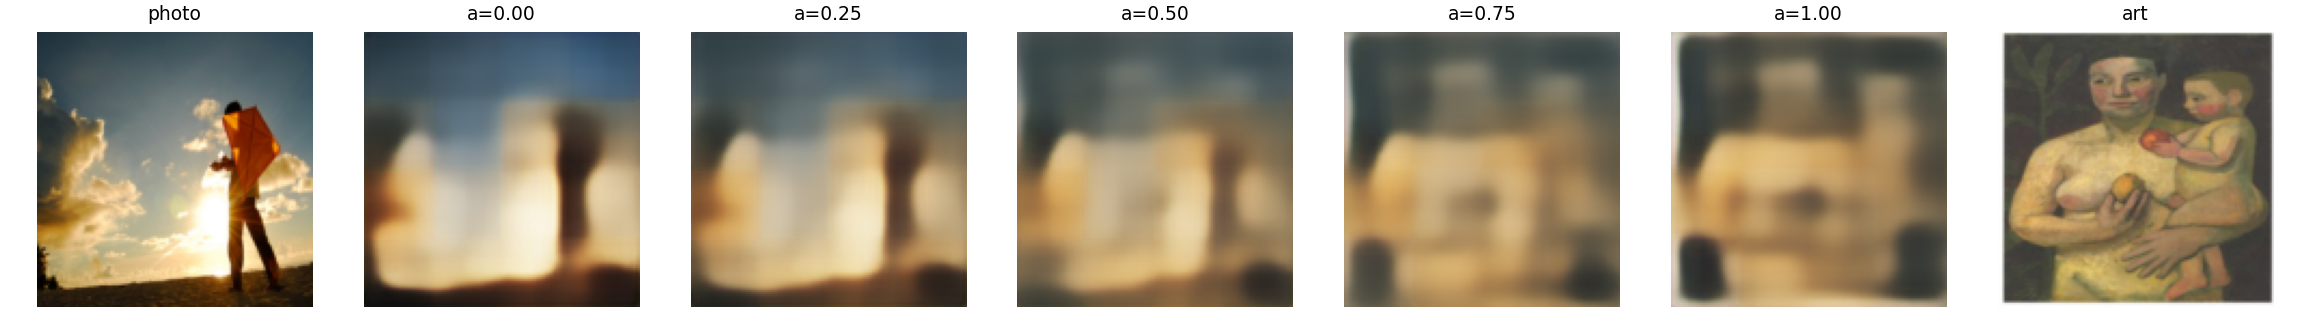
\includegraphics[width=0.95\textwidth]{visualizations/latent_interpolation.png}
    \caption{潜在空间插值生成的过渡风格图像}
    \label{fig:interp}
\end{figure}

\subsection*{6. 随机采样生成结果}
从标准正态分布中随机采样潜在向量，再分别指定目标域为照片域和艺术域，解码器即可生成新的图像。图 \ref{fig:gen-photo} 与图 \ref{fig:gen-art} 展示了模型在两个域上的随机生成结果。虽然细节真实感仍有提升空间，但结果已经体现出不同域在整体颜色和纹理风格上的差异。

\begin{figure}[H]
    \centering
    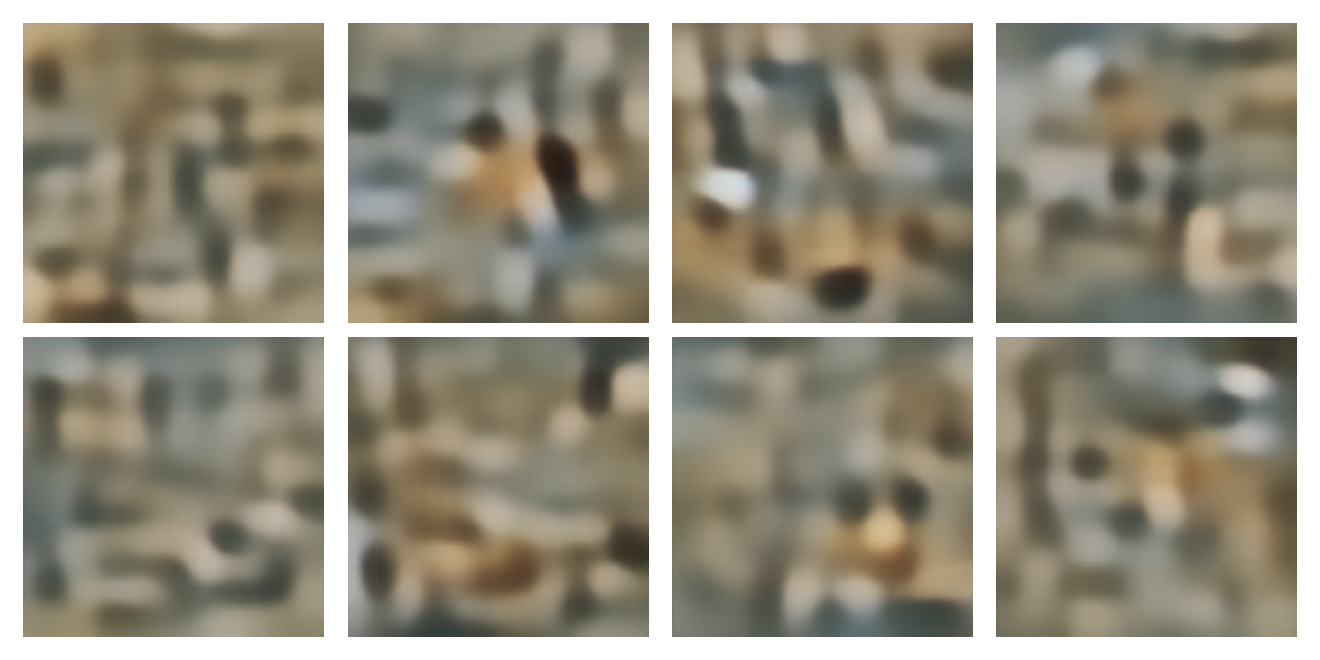
\includegraphics[width=0.9\textwidth]{visualizations/random_generation_photo.png}
    \caption{随机采样生成的照片域图像}
    \label{fig:gen-photo}
\end{figure}

\begin{figure}[H]
    \centering
    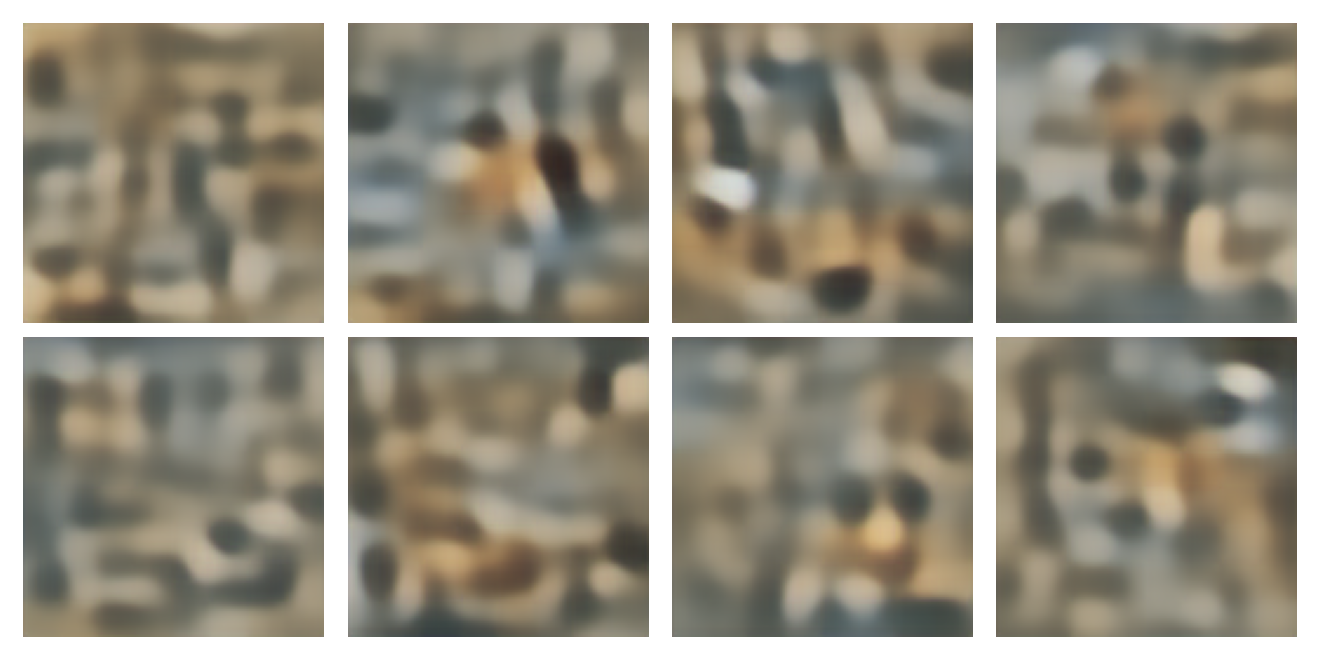
\includegraphics[width=0.9\textwidth]{visualizations/random_generation_art.png}
    \caption{随机采样生成的艺术域图像}
    \label{fig:gen-art}
\end{figure}

\section*{七、定量评估与结果分析}

\subsection*{1. MSE 指标}
根据实验要求，重建误差采用均方误差（MSE）进行度量。代码在测试阶段会统计模型在测试集上的总损失、重建损失、KL 损失以及 MSE，并在控制台打印结果。MSE 越小，说明重建图像在像素层面越接近真实图像；但需要注意的是，MSE 只能反映逐像素差异，不能完全衡量视觉风格转换质量。

\subsection*{2. FID 指标}
为了进一步从分布层面对生成图像质量进行评价，代码中额外预留了 FID 的计算函数。当安装 \texttt{torchmetrics} 和 \texttt{torch-fidelity} 后，可以分别计算 Photo$\rightarrow$Art 和 Art$\rightarrow$Photo 的 FID 分数。FID 越小，说明生成样本与目标域真实样本的分布越接近。由于本实验环境中 FID 依赖可能未完全安装，因此该部分作为可扩展评估模块给出。

\subsection*{3. 主观分析}
综合观察重建、迁移和随机生成结果，可以得到以下结论：
\begin{enumerate}
    \item 模型已经学到两类图像的整体结构信息，能够较稳定地重建场景轮廓与颜色分布；
    \item 在风格迁移中，写实图像能够转化出一定的印象派色彩与笔触效果，艺术图也能在一定程度上恢复到较平滑的照片域表现；
    \item VAE 生成图像仍存在一定模糊现象，局部细节、建筑边缘和人物纹理不够锐利，这与 VAE 的概率建模特性有关；
    \item 潜在空间插值结果较为平滑，说明模型提取到的隐变量具有较好的连续性和可操作性。
\end{enumerate}

\section*{八、存在的问题与改进方向}
尽管本实验已经完成了双向风格迁移与生成，但仍有若干不足：
\begin{itemize}
    \item 生成结果细节偏模糊，说明单纯的 VAE 在高分辨率图像生成方面仍受限；
    \item 目前的域条件信息较为简单，仅通过嵌入向量控制目标域，后续可以尝试更强的条件控制方式；
    \item FID 的稳定评估需要更多样本与更完善的环境支持；
    \item 若希望进一步提升视觉效果，可尝试引入感知损失、对抗损失，或采用 VQ-VAE、CVAE-GAN 等更强模型。
\end{itemize}

\section*{九、实验总结}
本实验基于 PyTorch 实现了一个面向双域图像的条件 VAE 模型，使用 COCO 写实照片和 WikiArt 印象派画作完成了图像重建、双向风格迁移、潜在空间插值与随机采样生成。实验表明，VAE 能够有效学习两类图像的潜在表示，并在保持整体场景结构的同时实现一定程度的风格转换。虽然生成结果在细节清晰度上仍有提升空间，但其潜在空间连续、训练稳定、可解释性较强，适合作为生成模型与风格迁移实验的基础方案。

\end{document}
